\documentclass{beamer}
\usepackage{../mysty}

\title{Week 07: Graphs}
\author{FanFly}
\date{April 19, 2020}

\begin{document}

\begin{frame}
  \titlepage
\end{frame}

\section{Eulerian Path}
\subsection{The Seven Bridges of K\"onigsberg}
\begin{frame}{The Seven Bridges of K\"onigsberg}
  The \emph{Seven Bridges of K\"onigsberg} is considered to be the first
  problem of graph theory. \pause \\[.5em]
  In this problem, people would like to know whether a citizen can take a walk
  through the town in such a way that each bridge would be crossed exactly
  once.
  \begin{figure}
    \includegraphics[scale=0.15]{bridges.jpg}
    \caption{The Seven Bridges of K\"oingsberg}
  \end{figure}
\end{frame}

\begin{frame}{Abstraction}
  The towns and bridges can be seen as vertices and edges in a graph.
  \begin{figure}
    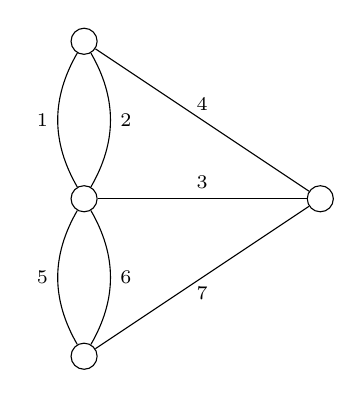
\begin{tikzpicture}
      \begin{scope}[every node/.style={circle,draw}]
        \node (A) at (0, 2) {};
        \node (B) at (0, 0) {};
        \node (C) at (0, -2) {};
        \node (D) at (3, 0) {};
      \end{scope}
      \begin{scope}[every node/.style={font=\scriptsize}]
        \draw (A) to[bend right=30] node[left] {1} (B);
        \draw (A) to[bend left=30] node[right] {2} (B);
        \draw (B) to node[above] {3} (D);
        \draw (A) to node[above] {4} (D);
        \draw (B) to[bend right=30] node[left] {5} (C);
        \draw (B) to[bend left=30] node[right] {6} (C);
        \draw (C) to node[below] {7} (D);
      \end{scope}
    \end{tikzpicture}
  \end{figure}
\end{frame}

\subsection{Graphs}
\begin{frame}{Graphs}
  In the following weeks, we are going to introduce some problems related to
  graphs. \pause \\[.5em]
  The definition of a graph is as follows.
  \begin{block}{Definition}
    A \emph{simple graph} is a pair $G = (V, E)$, where each component is as
    follows. \pause
    \begin{itemize}
      \item $V$ is a finite collection of \emph{vertices}. \pause
      \item $E$ is a collection of \emph{edges}, where each edge is of the form
      $e = \{u, v\}$ for some $u, v \in V$. \pause
    \end{itemize}
    If we allow a graph to have more than one edges that have the same
    endpoints, then the graph is called a \emph{multigraph}.
  \end{block}
\end{frame}

\subsection{Eulerian Path Problem}
\begin{frame}{Eulerian Path Problem}
  Now we can formalize the Seven Bridges of K\"onigsberg with new terminology.
  \pause
  \begin{itemize}
    \item A \emph{path} is a sequence of edges that joins a sequence of
    vertices. \pause
    \item An \emph{Eulerian path} is a path visiting each edge exactly once.
    \pause
  \end{itemize}
  Then a walk through the town in such a way that each bridge would be crossed
  exactly once is exactly an Eulerian path. \pause \\[1em]
  Thus, we have the following problem. \pause
  \begin{block}{Eulerian Path Problem}
    \begin{itemize}
      \item Input: A multigraph $G = (V, E)$.
      \item Output: Whether $G$ has an Eulerian path or not.
    \end{itemize}
  \end{block}
\end{frame}

\begin{frame}{The Solution to the Eulerian Path Problem}
  In fact, we have the following theorem, which simply solves the Eulerian path
  problem. \pause
  \begin{block}{Theorem}
    Let $G = (V, E)$ be a multigraph. \pause
    \begin{itemize}
      \item If each vertex in $G$ has an even degree, then $G$ has an Eulerian
      path that starts and ends on the same vertex. \pause
      \item If there are exactly two vertices of odd degree, then $G$ has an
      Eulerian path that starts on one of them and ends at the other. \pause
      \item If there are more than two vertices of odd degree, then $G$ has
      no Eulerian path. \pause
    \end{itemize}
  \end{block}
  The \emph{degree} of a vertex is the number of its incident edges.
\end{frame}

\begin{frame}{The Solution to the Eulerian Path Problem (cont.)}
  Thus, no one can take a walk through the town in such a way that each bridge
  would be crossed exactly once.
  \begin{figure}
    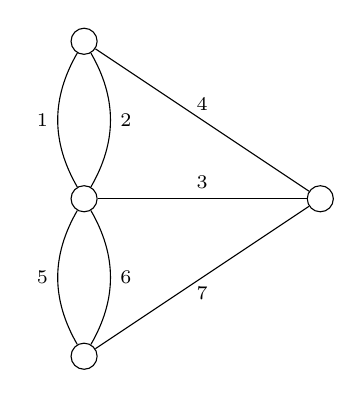
\begin{tikzpicture}
      \begin{scope}[every node/.style={circle,draw}]
        \node (A) at (0, 2) {};
        \node (B) at (0, 0) {};
        \node (C) at (0, -2) {};
        \node (D) at (3, 0) {};
      \end{scope}
      \begin{scope}[every node/.style={font=\scriptsize}]
        \draw (A) to[bend right=30] node[left] {1} (B);
        \draw (A) to[bend left=30] node[right] {2} (B);
        \draw (B) to node[above] {3} (D);
        \draw (A) to node[above] {4} (D);
        \draw (B) to[bend right=30] node[left] {5} (C);
        \draw (B) to[bend left=30] node[right] {6} (C);
        \draw (C) to node[below] {7} (D);
      \end{scope}
    \end{tikzpicture}
  \end{figure}
\end{frame}

\section{Representation of Graphs}
\subsection{Introduction}
\begin{frame}{Representation of Graphs}
  Now we can solve the Eulerian path problem. \pause \\[.5em]
  But how can we ``store'' a graph in an computer? \pause
  We need a \emph{data structure}! \pause \\[1em]
  We will focus on the efficiency of the following operations. \pause
  \begin{itemize}
    \item Initialize. \pause
    \item Check if an edge exists. \pause
    \item List all neighbors of a vertex. \pause
    \item List all edges.
  \end{itemize}
\end{frame}

\subsection{Edge List}
\begin{frame}[fragile]{Attempt \#1: Edge List}
  \begin{block}{Edge List}
    \scriptsize
    \begin{lstlisting}[gobble=4]
    n = 6
    edges = [[0, 1], [0, 2], [1, 3], [2, 3], [4, 5]]
    \end{lstlisting}
  \end{block}
\end{frame}

\subsection{Adjacency List}
\begin{frame}[fragile]{Attempt \#2: Adjacency List}
  \begin{block}{Adjacency List}
    \scriptsize
    \begin{lstlisting}[gobble=4]
    n = 6
    neighbor = [
        [1, 2],    # neighbor of vertex 0
        [0, 3],    # neighbor of vertex 1
        [0, 3],    # neighbor of vertex 2
        [1, 2],    # neighbor of vertex 3
        [5],       # neighbor of vertex 4
        [4]        # neighbor of vertex 5
    ]
    \end{lstlisting}
  \end{block}
\end{frame}

\subsection{Adjacency Matrix}
\begin{frame}[fragile]{Attempt \#3: Adjacency Matrix}
  \begin{block}{Adjacency Matrix}
    \scriptsize
    \begin{lstlisting}[gobble=4]
    n = 6
    matrix = [
        [False, True, True, False, False, False],
        [True, False, False, True, False, False],
        [True, False, False, True, False, False],
        [False, True, True, False, False, False],
        [False, False, False, False, False, True],
        [False, False, False, False, True, False]
    ]
    \end{lstlisting}
  \end{block}
\end{frame}

\section{Exercises}
\subsection{\#1}
\begin{frame}{Exercise \#1}
  A \emph{complete graph} is a graph in which each pair of vertices is
  connected by an edge. \pause \\[.5em]
  What is the number of edges of an $n$-vertex complete graph? \\
  (By the way, the $n$-vertex complete graph is denoted by $K_n$). \pause
  \begin{block}{Solution}
    There are $n(n-1)/2$ edges in $K_n$.
  \end{block}
\end{frame}

\subsection{\#2}
\begin{frame}{Exercise \#2}
  Let $G = (V, E)$ be a graph with $|V| = n$. \pause \\[.5em]
  How much time does it take to find the degree of a vertex in $V$
  if $G$ is stored as an adjacency matrix? \pause
  \begin{block}{Solution}
    It takes $\Theta(n)$ time.
  \end{block}
\end{frame}

\subsection{\#3}
\begin{frame}{Exercise \#3}
  A \emph{coloring} of a graph is a labeling of vertices with colors such that
  no two adjacent vertices have the same color. \pause \\[.5em]
  What is the minimum number of colors needed to color $K_5$? \pause
  \begin{block}{Solution}
    We need 5 colors to color $K_5$.
  \end{block}
\end{frame}

\end{document}